\section{Theory}

\subsection{Actuator Modeling}
    \subsubsection{DC Motor Model}



    \subsubsection{BLDC Motor Model}


    \begin{figure}[H]
        \centering
        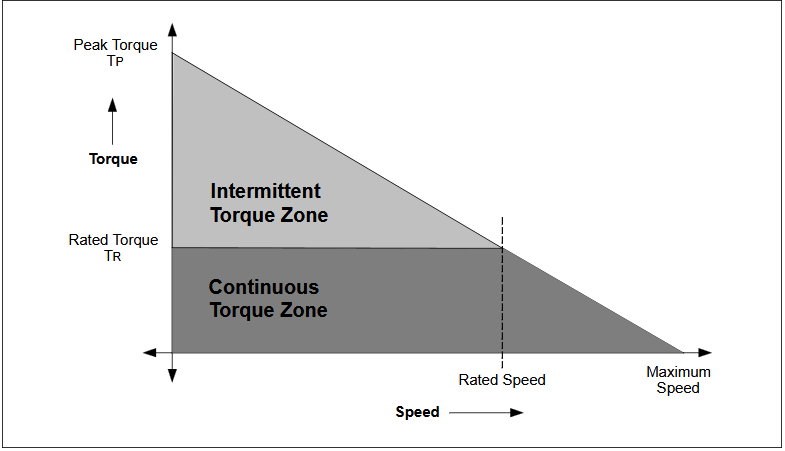
\includegraphics[width=0.5\textwidth]{Images/stolen_BLDC_torque_speed.png}
        \caption{Torque-speed characteristics of a BLDC motor. TODO: Replace with an image that isn't stolen, and that we are allowed to use. }
        \label{fig:bldc_torque_speed}
    \end{figure}

    \subsubsection{Gear Transmission Friction Model}

    Although electric motors for robotics are available for a wide power range, they are often too high speed and low power to do any useful work. For this reason, it is often necessary to use a gear transmission to increase the torque and reduce the speed of the motor. 

    In the presence of a geared transmission, assuming no power loss, the output torque and velocity of a geared motor are given by equation \ref{eq:gear_torque} and equation \ref{eq:gear_velocity}, respectively, where $N$ is the gear ratio, $\tau_{in}$ is the input torque, $\tau_{out}$ is the output torque, $w_{in}$ is the input velocity, and $w_{out}$ is the output velocity \cite{modern_robotics_book}.

    \begin{equation}
        \label{eq:gear_torque}
        w_ {out} = \frac{w_{in}}{N}
    \end{equation}

    \begin{equation}
        \label{eq:gear_velocity}
        \tau_{out} = N\tau_{in}
    \end{equation}

    In reality, however, there is always some power loss in the transmission. A common way to model this is to use friction model consisting of a viscous friction term and a Coulomb friction term \cite{modern_robotics_book}. The viscous friction term is proportional to the velocity of the transmission, and the Coulomb friction term is a constant friction torque that must be overcome before the transmission starts moving. The total friction torque is the sum of these two terms, as seen in equation \ref{eq:friction_torque}. It is also possible to drop one or the other of these terms, depending on the application \cite{modern_robotics_book}.

    \begin{equation}
        \label{eq:friction_torque}
        \tau_{friction} = b_{viscous}\dot{\theta} + b_{coulomb}\text{sign}(\dot{\theta})  
    \end{equation}

    In addition to friction, heavily gearing motors can lead to a very high apparent rotor inertia. If one looks at equation \ref{eq:rotor_kinetic_energy}, it is clear that the apparent rotor inertia is proportional to the square of the gear ratio \cite{modern_robotics_book}. This can lead to a very high apparent rotor inertia, which can often be problematic to robotic applications. This is especially the case for cases with contact forces, as the high apparent rotor inertia can lead to very stiff and damaging collisions \cite{proprioceptive}.

    \begin{equation}
        \label{eq:rotor_kinetic_energy}
        K = \frac{1}{2}{I}_{rotor}(G\dot\theta)^2 = \frac{1}{2}{I}_{rotor}G^2(\dot\theta)^2 = \frac{1}{2}I_{apparent}(\dot\theta)^2
    \end{equation}

\subsection{Spring Modeling}
\label{sec:spring_theory}
Springs are mechanical devices that store and release energy when subjected to displacement. There are two main types of springs: extension springs and torsion springs.

Extension springs are designed to operate with a tension load, meaning they extend as the load is applied. The force exerted by an extension spring is proportional to the displacement from its equilibrium position, following Hooke's Law, which is given by:
\begin{equation}
    F = -kx
\end{equation}
where \( F \) is the force exerted by the spring, \( k \) is the spring constant, and \( x \) is the displacement from the equilibrium position. The potential energy stored in an extension spring is given by:
\begin{equation}
    U = \frac{1}{2}kx^2
\end{equation}

Torsion springs, on the other hand, are designed to operate with a rotational or twisting load. They exert a torque that is proportional to the angular displacement from their equilibrium position. The torque generated by a torsion spring is given by:
\begin{equation}
    \tau = -k\theta
\end{equation}
where \( \tau \) is the torque, \( k \) is the torsion spring constant, and \( \theta \) is the angular displacement. The potential energy stored in a torsion spring is given by:
\begin{equation}
    U = \frac{1}{2}k\theta^2
\end{equation}

Both types of springs are widely used in various mechanical systems to provide force or torque, absorb shock, and store energy.

\subsection{Spring-Damper Systems}

\subsection{Kinematics, Jacobians, and Virtual Work}
    \subsubsection{Robot Kinematics}
    \label{sec:robot_kinematics}
Consider a robotic link arm existing in $\mathbb{R}^2$ consisting of $n$ links, each with a length $l_i$ and a joint angle $q_i$. The position of the end-effector is given by the vector $\mathbf{x} = [x, y]^T$, where $x$ and $y$ are the coordinates of the end-effector in the global coordinate system. Using simple trigonometry, the position of the end-effector can be expressed as a function of the joint angles and link lengths as seen in equation \ref{eq:robot_kinematics}. 
Axes and joint angles corresponding to the expression in equation \ref{eq:robot_kinematics} can be seen in figure \ref{fig:robotic_link_arm}. 

\begin{equation}
    \label{eq:robot_kinematics}
    \mathbf{x} = \begin{bmatrix}
        x \\
        y
    \end{bmatrix} = \begin{bmatrix}
        \sum_{i=1}^{n} l_i \cos(q_i) \\
        \sum_{i=1}^{n} l_i \sin(q_i)
    \end{bmatrix}
\end{equation}

\begin{figure}[H]
    \centering
    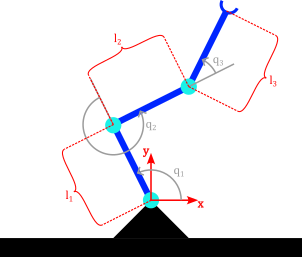
\includegraphics[width=0.5\textwidth]{Images/manipulator_inkscape_Layer 1.png}
    \caption{Illustration of a 3 link robotic link arm in $\mathbb{R}^2$ with $n$ links.}
    \label{fig:robotic_link_arm}
\end{figure}


    \subsubsection{Jacobian Matrix}

As described in section \ref{sec:robot_kinematics}, the position of the end-effector can be expressed as a function of the joint angles and link lengths. In robotics, it is often useful to express the relationship between infinitesimal changes in the joint angles and the resulting change in the end-effector position. As can be seen in equation \ref{eq:infinitesimal_change}, infinitesimal changes in variables $\delta y$ and $\delta x$ can be described by means of the partial derivative \cite{modsim}. If this is compared to the definition of the jacobian in equation \ref{eq:jacobian}, it is clear that the jacobian matrix $\mathbf{J}$ can be used to map infinitesimal changes in joint angles to changes in the end-effector position, as illustrated in equation \ref{eq:jacobian_pos_mapping}. The limit of an infinitesimal change over an infinitesimal time interval is a derivative, and thus by dividing each side in equation \ref{eq:jacobian_pos_mapping} by $\delta t$, one arrives at the expression in equation \ref{eq:jacobian_speed_mapping}, by which the jacobian can be used to map joint velocities to end-effector velocities.

\begin{equation}
    \label{eq:infinitesimal_change}
    \delta  y = \frac{\partial y}{\partial x} \delta x
\end{equation}

\begin{equation}
    \label{eq:jacobian}
    \mathbf{J} = \begin{bmatrix}
        \frac{\partial x}{\partial q_1} & \frac{\partial x}{\partial q_2} & \cdots & \frac{\partial x}{\partial q_n} \\
        \frac{\partial y}{\partial q_1} & \frac{\partial y}{\partial q_2} & \cdots & \frac{\partial y}{\partial q_n}
    \end{bmatrix}
\end{equation}

\begin{equation}
    \label{eq:jacobian_pos_mapping}
    \mathbf{\delta x} = \mathbf{J}\mathbf{\delta q}
\end{equation}

\begin{equation}
    \label{eq:jacobian_speed_mapping}
    \mathbf{\dot x} = \mathbf{J}\mathbf{\dot q}
\end{equation}

    \subsubsection{Force/Torque Mapping}
    \label{sec:force_torque_mapping}

    Consider a general robotic manipulator, such as the one illustrated in figure \ref{fig:robotic_link_arm}, but with an arbitrary amount, $n$, of joints and links. Using the principle of conservation of power, one arrives at the formulation found in equation \ref{eq:power_conservation}.

    \begin{equation}
        \text{power at the joints} = \text{(power to move the robot)} + \text{(power at the end-effector)}
        \label{eq:power_conservation}
    \end{equation}
    
    As the power used to move the robot approaches zero, ...

    Consider a robotic manipulator with $n$ joints, each with a joint angle $q_i$ and a joint torque $\tau_i$. The position of the end effector for such a system is given by equation \ref{eq:robot_kinematics}, and thus the formula in equation \ref{eq:jacobian_speed_mapping} can be used to map joint velocities to end effector velocities. 

    TODO: Derive equation \ref{eq:force_torque_mapping} by either power balance, or virtual work. 

    \begin{equation}
        \label{eq:force_torque_mapping}
        \tau = J^T F
    \end{equation}

\subsection{Numerical Solvers}
\label{sec:numerical_solvers}

Although a detailed review of numerical solvers and the associated theory is beyond the scope of this theory section, it is worth mentioning that numerical simulation of contact dynamics is particularly challenging. This is due to the discontinuities and high-frequency events that occur during contact. These dynamics often require the use of stiff solvers to accurately capture the rapid changes in forces and velocities \cite{stiff_contact_ODE_1}\cite{stiff_contact_ODE_2}. Stiff solvers are designed to handle problems with widely varying timescales, ensuring stability and accuracy in the simulation of contact events. Without the use of stiff solvers, simulations can become unstable or fail to converge, leading to inaccurate results. Examples of stiff solvers include the well known ode15s and ode23s solvers in MATLAB, which are specifically designed to handle stiff ordinary differential equations \cite{MATLAB_ODE}. 



\subsection{Linear Least Squares Regression}
Linear least squares regression is a method for finding the best-fitting line through a set of points by minimizing the sum of squared residuals. Given a set of observations \((x_i, y_i)\) and a linear model \(y = X\beta\), where \(X\) is the matrix of input variables and \(\beta\) contains the model parameters, the residual \(r_i\) for each observation is:

\[
r_i = y_i - X_i\beta
\]

The sum of squared residuals \(S\) is then:

\[
S = \sum_{i=1}^n r_i^2 = (y - X\beta)^T(y - X\beta)
\]

To minimize \(S\), we take its derivative with respect to \(\beta\) and set it to zero:

\[
\frac{\partial S}{\partial \beta} = -2X^T(y - X\beta) = 0
\]

Solving for \(\beta\) yields the normal equations:

\[
X^TX\beta = X^Ty
\]

The solution is therefore:

\[
\beta = (X^TX)^{-1}X^Ty
\]

This solution minimizes the sum of squared residuals and provides the optimal parameters \(\beta\) in the least squares sense.

\subsection{Inverse Kinematics}
Inverse kinematics solves for joint angles that achieve a desired end-effector pose. For a planar two-link manipulator with link lengths \(L_1\) and \(L_2\), given a desired end-effector position \((x,y)\), the joint angles \(\theta_1\) and \(\theta_2\) can be found analytically.

From the law of cosines, \(\theta_2\) is:

\[
\theta_2 = \pm \arccos\left(\frac{x^2 + y^2 - L_1^2 - L_2^2}{2L_1L_2}\right)
\]

The angle \(\theta_1\) is then:

\[
\theta_1 = \arctan2(y,x) - \arctan2(L_2\sin(\theta_2), L_1 + L_2\cos(\theta_2))
\]

The ± in the equation for \(\theta_2\) indicates that two solutions exist for most end-effector positions - one with the second joint angle positive and one negative. When \(L_1 = L_2\), a singularity occurs at \((0,0)\) where infinite solutions exist. At the workspace boundary where \(x^2 + y^2 = (L_1 + L_2)^2\), only one solution exists.


